\documentclass[12pt,a4paper]{article}
\usepackage[utf8]{inputenc}
\usepackage[english]{babel}
\usepackage{amsmath}
\usepackage{amsfonts}
\usepackage{amssymb}
\usepackage{graphicx}
\usepackage{hyperref}
\usepackage{xcolor}
\usepackage{listings}

\setlength\parindent{0pt}

\author{slarticodefast \\ \href{https://github.com/slarticodefast}{github.com/slarticodefast}}
\title{\vspace{-4.0cm}SS14 throwing system improvements}

\begin{document}
\maketitle
\begin{figure}[t]
\centering
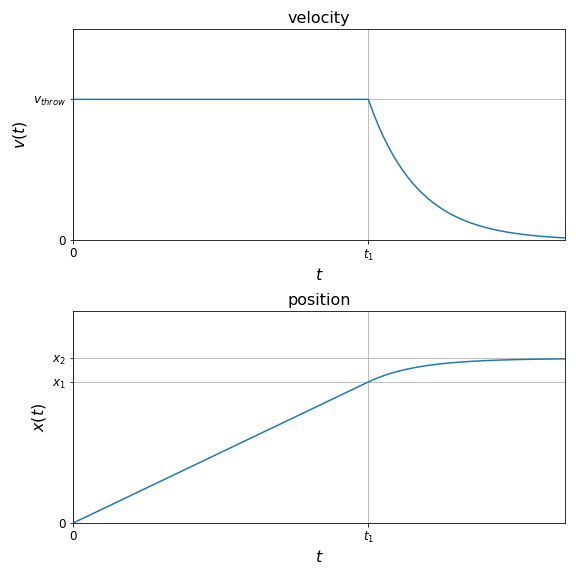
\includegraphics[width=0.8\linewidth]{throwing.png}
\end{figure}
\sloppy{
Friction is calculated in the \texttt{ReduceLinearVelocity} function in \texttt{TileFrictionController.cs} using the following change in velocity}:

\begin{align}
 &                 & v'         &= v + dv& \\
 &                 &            &= v \cdot (1 - F \cdot dt)& \\
 &\Leftrightarrow  & dv         &= -F \cdot v \cdot dt& \\
 &\Leftrightarrow  & \dot{v}(t) &= \frac{dv}{dt} = -F \cdot v(t)& 
\end{align}
where $F$ is the friction given by the product of the \texttt{TileFrictionModifier} cvar, the tile friction given in \texttt{TileFrictionController.cs} and the body modifier set via \texttt{TileFrictionEvent}.
\vskip 0.5cm
This differential equation is solved by an exponential decay
\begin{equation}
v(t)=v_{throw}\cdot \exp(-F \cdot(t-t_1))
\end{equation}
where $v_{throw}$ is the initial velocity and $t_1$ the starting time of the decay. When thrown, items are first set to be in the air for the time $t_1$, during which they receive no friction and therefore stay at constant velocity. When landing, a \texttt{LandEvent} is raised. Note that the slowdown is independent of the object's mass.
\vskip 0.5cm
The velocity and position over time are plotted below. We calculate the distance from the starting position when landing via
\begin{equation}
d_1=v_{throw} \cdot t_1
\end{equation}
After landing the item will slide on the ground until it stops moving at position $d_2$. While from a mathematical point of view the item will never completely stop and never reaches $d_2$ exactly, numerically its velocity is set to zero below a certain threshold. By integrating the velocity we calculate
\begin{align}
d_2 &= d_1 + \int_{t_1}^{\infty} v_{throw} \cdot \exp(-F \cdot(t-t_1))dt\\
&= d_1 + \Big[-\frac{v_{throw}}{F} \cdot \exp(-F \cdot(t-t_1)\Big]_{t_1}^{\infty}\\
&= d_1 - \frac{v_{throw}}{F}\cdot \exp(-\infty) + \frac{v_{throw}}{F} \exp(0)\\
&= d_1 + \frac{v_{throw}}{F}
\end{align}
We rearrange this to
\begin{align}
d_2 &= v_{throw} \cdot t_1 + \frac{v_{throw}}{F}\\
&= v_{throw}\cdot\Big(t_1+\frac{1}{F}\Big)\\
\Leftrightarrow \quad v_{throw} &= \frac{d_2}{\big(t_1+\frac{1}{F}\big)}
\end{align}
With this formula we are able to calculate the required throwing speed $v_{throw}$ for a desired throwing distance $d_2$ (given by the player's cursor position).The time $t_1$ is a free parameter. If it is too low, the item will slide on the floor for most of the distance. If it is too high, the item will be thrown very slowly in a high arc. As a reasonable choice we set
\begin{equation}
t_1 = p_{flyTime} \cdot \frac{d_2}{v_{base}}
\end{equation}
where $p_{flyTime}$ is the percentage of time the item would be  in the air if it would not slow down after landing, and $v_{base}=10$ is the corresponding base throwing speed given by the \texttt{HandsComponent}. We choose $p_{flyTime}=0.8$ so that the item is in the air for approximately 80\% of the time of the throw.
\vskip 0.5cm
For throwing weapons like spears or hypodarts we want slightly different throwing mechanics. Using the above throwing parameters, the spear would slowly land at the opponents feet if the player's cursor is directly above the opponent. Therefore we use
\begin{align*}
t_1&=\frac{d_2}{v_{base}}\\
v_{throw}&=v_{base}
\end{align*}
instead. This makes the item land at the cursor position and slide a little further along the ground from there. To select which items should follow this behavior we add a new \texttt{LandAtCursorComponent}. This should be added to all throwing weapons that pierce the opponent or are supposed to land (but not stop) exactly at his position.
\end{document}